\documentclass[usenames,dvipsnames]{beamer}
%-------------------------------------------------------
% THEME SETTINGS
%-------------------------------------------------------
\usetheme[progressstyle=movingCircCnt]{Feather}
\setbeamercolor{Feather}{fg=black!30,bg=black}
\setbeamercolor{structure}{fg=black}
\setbeamercolor{block body example}{bg=black!5!white}
\setbeamercolor{block title example}{fg=white,bg=black!40!white}


\usepackage{amsmath,amssymb,amsfonts}
\usepackage{cite}
\usepackage{multirow}
\usepackage{booktabs}
\usepackage{hhline}
\usepackage{multicol}
%\usepackage{showframe}

\usepackage{tikz}
%\usetikzlibrary{patterns}
\usetikzlibrary{patterns,arrows,decorations.pathmorphing,backgrounds,shadows,positioning,fit,shapes,matrix,calc,shapes.multipart,arrows.meta}
\usepackage[simplified]{pgf-umlcd}
\usepackage{xpatch} % Needed for patching pgf-umlcd
\usepackage{xparse} % Needed for patching pgf-umlcd
\usepackage{color,soul} % for \hl
\definecolor{dark-yellow}{RGB}{219, 212, 143}
\definecolor{dark-green}{RGB}{36,84,36}
\definecolor{my-gray}{gray}{0.85}
\sethlcolor{dark-yellow}



\usepackage{wrapfig}
\usepackage{listings}
\usepackage{adjustbox}
\usepackage{graphicx}
\usepackage{caption}
\usepackage{multirow}
\usepackage{subcaption}
\usepackage{stmaryrd}
\usepackage{hyperref}
\usepackage{float}
\usepackage{textcomp}
\usepackage{tikz-qtree,tikz-qtree-compat}

\newcommand*{\emphColorSlide}[1]{\textcolor{ForestGreen}{\textbf{#1}}}
\newcommand*{\emphSlide}[1]{\textcolor{ForestGreen}{\textbf{#1}}}

\newcommand*{\lowEmph}[1]{\textcolor{NavyBlue}{\textbf{#1}}}
\newcommand*{\subt}{\textcolor{NavyBlue}{\textbf{<:}}}
\newcommand*{\supt}{\textcolor{NavyBlue}{\textbf{:>}}}



\newcommand{\dataflow}{data-flow}
\newcommand{\Dataflow}{Data-flow}
\newcommand{\code}[1]{\texttt{\lstinline[basicstyle=\normalsize\ttfamily,identifierstyle={\normalsize},commentstyle={\normalsize\itshape},keywordstyle={\normalsize\bfseries},ndkeywordstyle={\normalsize},stringstyle={\normalsize\ttfamily},numberstyle={\normalsize}]!#1!}}
\newcommand{\CFG}{CFG}
\newcommand{\intraj}{\emphColorSlide{\textsc{Intra}J}}
\newcommand{\intrajs}{\emphColorSlide{\textsc{IntraJ}}}
\newcommand{\intracfgs}{\emphColorSlide{\textsc{IntraCFG}}}
\newcommand{\jastaddjintraflow}{\textsc{jastaddj-intraflow}}
\newcommand{\jji}{\code{JJI}}
\newcommand{\jastadd}{\textsc{JastAdd}}
\newcommand{\extendj}{\textsc{ExtendJ}}
\newcommand{\cG}{\mathcal{G}}
\newcommand{\cV}{\mathcal{V}}
\newcommand{\cE}{\rightarrowtail}
\newcommand{\cP}{\mathcal{P}}
\newcommand{\cM}{\mathcal{M}}


\newcommand{\mSyn}{\ensuremath{\uparrow}}
\newcommand{\mInh}{\ensuremath{\downarrow}}
\newcommand{\mHOA}{\ensuremath{\rightarrow}}
\newcommand{\mColl}{\ensuremath{\square}}
\newcommand{\mCirc}{\ensuremath{\circlearrowleft}}

\newcommand{\Abase}[1]{\textcolor{ATGsym}{\mbox{\umlcode{#1}}}}
\newcommand{\Asyn}[1]{\textcolor{ATGsym}{\mbox{\mSyn{}\umlcode{#1}}}}
\newcommand{\Ainh}[1]{\textcolor{ATGsym}{\mbox{\mInh{}\umlcode{#1}}}}
\newcommand{\Ahoa}[1]{\textcolor{ATGsym}{\mbox{\mHOA{}\umlcode{#1}}}}
\newcommand{\Acoll}[1]{\textcolor{ATGsym}{\mbox{\mColl{}\umlcode{#1}}}}
\newcommand{\Acirc}[1]{\textcolor{ATGsym}{\mbox{\mCirc{}\umlcode{#1}}}}

\newcommand{\umlcode}[1]{\textrm{#1}}  % Style of code used in UML fragments
\newcommand{\astnodestyle}{\ttfamily\color{magenta}}
\newcommand{\astnode}[1]{\texttt{\textcolor{magenta}{#1}}}  % Style used for AST node types

\newcommand{\ASTUnrestricted}{AST-unrestricted}
\newcommand{\ParentFirst}{Parent-First}

\newcommand{\project}[1]{\textsc{#1}}
\newcommand{\tool}[1]{\textsc{#1}}

% can't get fbox to work reliably in the UML code, and adjustbox and nested \tikz don't work at all
%\newcommand{\dfapi}{\textsf{\setlength{\fboxsep}{0pt}\fcolorbox{blue}{white}{df-api}}}
\newcommand{\dfapi}{\textbf{\textcolor{black}{[df-api]}}}
\newcommand{\nameapi}{\textbf{\textcolor{black}{[name-api]}}}

\newcommand{\frameworkname}{\textsc{Intra}CFG}
\newcommand{\intracfg}{\textsc{\frameworkname}}

\newcommand{\node}{\mathsf{n}}
\newcommand{\Null}{\mathtt{NULL}}
\newcommand{\Notnull}{\mathtt{NOTNULL}}
\newcommand{\gen}{\mathtt{gen}}
\renewcommand{\kill}{\mathtt{kill}}

\newcommand{\In}{\mathtt{in}}
\newcommand{\Out}{\mathtt{out}}
\newcommand{\Use}{\mathtt{use}}
\newcommand{\Def}{\mathtt{def}}
\newcommand{\tf}{f_t}
\newcommand{\mCi}[1]{ { \textcolor{black!30}{\tiny \pm\text{#1}}}}%Condifdence interval

\newcommand{\CR}[1]{\textbf{[}\textcolor{blue!60!black}{\textbf{CR:} #1}\textbf{]}}
\newcommand{\Ckw}[1]{\texttt{\textbf{#1}}}
\newcommand{\auxlabel}[1]{{\scriptsize{$\textrm{\texttt{#1}}$}}}
\newcommand{\auxlabeli}[2]{{\scriptsize{$\textrm{\texttt{#2}}_{#1}$}}}
\newcommand{\auxlabelbox}[1]{\tikz[baseline=-0.7ex] \node[rectangle, minimum width=0, thin, draw, rounded corners, fill=white, inner sep=2pt, outer sep=0pt] (N) {\auxlabel{#1}};}
\newcommand{\auxlabelboxhoa}[1]{\tikz[baseline=-0.7ex] \node[rectangle, dashed,minimum width=0, thin, draw, rounded corners, fill=white, inner sep=2pt, outer sep=0pt] (N) {\auxlabel{#1}};}

%\newcommand{\auxlabelboxi}[2]{\tikz \node[rectangle, minimum width=0, thin, draw, rounded corners, fill=white] {\auxlabeli{#1}{#2}};}

\newcommand{\Prod}{::=}
\newcommand{\terminal}[1]{\textcolor{green!50!black}{\textit{#1}}}
\newcommand{\vmetavar}[1]{\textcolor{cyan!30!black}{\textsf{\textbf{#1}}}}
\newcommand{\vcode}[1]{\textsf{\textcolor{green!35!black}{{#1}}}}
\newcommand{\vterminal}[1]{\vcode{#1}}
\newcommand{\nta}[1]{\ensuremath{\textit{#1}}}
\newcommand{\tuple}[1]{\ensuremath{\langle #1 \rangle}}
\newcommand{\nt}[1]{\ensuremath{\tuple{\hspace{-0.02cm}\nta{#1}\hspace{0.02cm}}}}
\newcommand{\VB}{\ |\ }
\newcommand{\Gcomment}[1]{\textrm{\textcolor{black!50!white}{({#1})}}}
\newcommand{\sem}[1]{\ensuremath{\llbracket #1 \rrbracket}}
%\newcommand{\semNPA}[1]{\ensuremath{\sem{#1}_{\textit{NPA}}}}
\newcommand{\semNPA}[1]{\ensuremath{\sem{#1}}}

\newcommand{\listingsfontsize}{\scriptsize}

\newcommand{\NAmark}{\multicolumn{1}{c}{\textcolor{black!40!white}{-}}}
\newcommand{\NAmarkR}{\multicolumn{1}{c|}{\textcolor{black!40!white}{-}}}
\newcommand{\Tcenter}[1]{\multicolumn{1}{c}{#1}}
\newcommand{\TcenterR}[1]{\multicolumn{1}{c|}{#1}}
\newcommand{\succarrow}{\tikz[baseline=-0.7ex] \draw[succarrow, thick, -{Stealth[scale=0.9, inset=0pt, angle'=45]}] (0,0) -- (0.3,0.0);}

\colorlet{hlgreen}{green}
\colorlet{hlorange}{orange}
\colorlet{hlgreenhalf}{green!50!white}
\colorlet{hlorangehalf}{orange!50!white}
\colorlet{npagrey}{gray!10!white}

\DeclareRobustCommand{\hlgreen}[1]{{\sethlcolor{hlgreenhalf}\hl{#1}}}
\DeclareRobustCommand{\hlorange}[1]{{\sethlcolor{hlorangehalf}\hl{#1}}}

\definecolor{ATGsym}{HTML}{206010}

\definecolor{SQ}{HTML}{0080ff}
\definecolor{JJI}{HTML}{ff0080}
\definecolor{IJnonH}{HTML}{004010}
\definecolor{IJH}{HTML}{00ff20}

\definecolor{succarrow}{HTML}{4e90e2}	% adapted from RunningExample.tex

\definecolor{lightblue}{HTML}{006699}		%#006699
\definecolor{lightgreen}{HTML}{669900}		%#669900
\lstdefinelanguage{JastAdd}{
  %keyword1&2&6
  morekeywords = [1]{class, extends, private, void,new},
  %keyword3
  morekeywords = [2]{this,null}, %JASTADD keywords
  %keyword4
  morekeywords = [3]{return}, %ASTnode typess
  %keyword5
  morekeywords = [4]{},
  keywordstyle = [1]\color{lightblue},
  keywordstyle = [2]\color{lightgreen},
%  keywordstyle = [1]\bfseries,
%  keywordstyle = [2]\bfseries,
  keywordstyle = [3]\astnodestyle,
  keywordstyle = [4]\color{orange},
  sensitive = true,
  morecomment = [l]{//},
  morecomment = [s]{/*}{*/},
  morecomment = [s]{/**}{*/},
  commentstyle = \color{gray},
  morestring = [b]",
  morestring = [b]',
  stringstyle = \color{purple}
}
\lstset{
  backgroundcolor =\color{npagrey},
  basicstyle=\listingsfontsize\ttfamily,
  identifierstyle={\listingsfontsize},
  commentstyle={\listingsfontsize\itshape},
  keywordstyle={\listingsfontsize\bfseries},
  ndkeywordstyle={\listingsfontsize},
  stringstyle={\listingsfontsize\ttfamily},
  frame={tb},
  breaklines=true,
  breakatwhitespace=true, %To avoid linebreaks between \code{} and comma.
  columns=[l]{fullflexible},
  numbers=none,
  numberstyle={\listingsfontsize},
  stepnumber=1,
  mathescape,
	escapeinside     = {!}{!}, %General escape does not seem to work in lstinline/GH.
}

\makeatletter
\pgfdeclareshape{topbottombox}{
  \inheritsavedanchors[from=rectangle]
  \inheritanchorborder[from=rectangle]
  \inheritanchor[from=rectangle]{center}
  \inheritanchor[from=rectangle]{base}
  \inheritanchor[from=rectangle]{north}
  \inheritanchor[from=rectangle]{north east}
  \inheritanchor[from=rectangle]{east}
  \inheritanchor[from=rectangle]{south east}
  \inheritanchor[from=rectangle]{south}
  \inheritanchor[from=rectangle]{south west}
  \inheritanchor[from=rectangle]{west}
  \inheritanchor[from=rectangle]{north west}
  \backgroundpath{
    %  store lower right in xa/ya and upper right in xb/yb
    \southwest \pgf@xa=\pgf@x \pgf@ya=\pgf@y
    \northeast \pgf@xb=\pgf@x \pgf@yb=\pgf@y
    \pgfpathmoveto{\pgfpoint{\pgf@xa}{\pgf@ya}}
    \pgfpathlineto{\pgfpoint{\pgf@xb}{\pgf@ya}}
    \pgfpathmoveto{\pgfpoint{\pgf@xa}{\pgf@yb}}
    \pgfpathlineto{\pgfpoint{\pgf@xb}{\pgf@yb}}
 }
}
\makeatother


% Patch UML package pgf-umlcd to be able to write abstract grammar as class name.
\ExplSyntaxOn
\NewDocumentCommand{\defineclassname}{m}
 {
  \tl_set:Nn \umlcdClassName { #1 }
  \tl_set_eq:NN \umlcdClassNameString \umlcdClassName
  \tl_replace_all:Nfn \umlcdClassName { \char_generate:nn { `_ } { 8 } } { \_\kern1pt }
 }
\cs_generate_variant:Nn \tl_replace_all:Nnn { Nf }
\ExplSyntaxOff
\xpatchcmd{\classAndInterfaceCommon}
 {\def\umlcdClassName}
 {\defineclassname}
 {}{}
\xpatchcmd{\endclass}
 {(\umlcdClassName)}
 {(\umlcdClassNameString)}
 {}{\ddt}
\xpatchcmd{\endinterface}
 {(\umlcdClassName)}
 {(\umlcdClassNameString)}
 {}{\ddt}
\xpatchcmd{\endabstractclass}
 {(\umlcdClassName)}
 {(\umlcdClassNameString)}
 {}{\ddt}
\xpatchcmd{\endobject}
 {(\umlcdClassName)}
 {(\umlcdClassNameString)}
 {}{\ddt}
\xpatchcmd{\endclassAndInterfaceCommon}
 {(\umlcdClassName)}
 {(\umlcdClassNameString)}
 {}{\ddt}
\xpatchcmd{\endclassAndInterfaceCommon}
 {(\umlcdClassName)}
 {(\umlcdClassNameString)}
 {}{\ddt}
\xpatchcmd{\endclassAndInterfaceCommon}
 {(\umlcdClassName)}
 {(\umlcdClassNameString)}
 {}{\ddt}

\newbool{ANON}
%\booltrue{ANON}
\boolfalse{ANON}
\newcommand{\anon}[2]
{\ifbool{ANON}{
   #1
}{
   #2
}}



\makeatletter
\renewcommand\@makefnmark{\hbox{\@textsuperscript{\usebeamercolor[fg]{footnote mark}\usebeamerfont*{footnote mark}[\@thefnmark]}}}
\renewcommand\@makefntext[1]{\@textsuperscript{\usebeamercolor[fg]{footnote mark}\usebeamerfont*{footnote mark}[\@thefnmark]}\usebeamerfont*{footnote} #1}
\makeatother

%Modify the Title display on frame
\makeatletter
\patchcmd\beamer@@tmpl@frametitle{\insertframetitle}{{\footnotesize \insertsection~\emphColorSlide{\insertsubsection}~\\} \textbf{\insertframetitle}}{}{}
\makeatother
%Add space to the footline
\makeatletter
\patchcmd{\beamer@calculateheadfoot}{\advance\footheight by 4pt}{\advance\footheight by 8pt}{}{}
\makeatother

%NO HEAD LINE
\makeatletter
\newenvironment{noheadline}{
	\setbeamertemplate{headline}[default] {}
	\setfootline
}{}
\makeatother

%Slide with  Section title
%\AtBeginSection[]{
%	\begin{noheadline}
%	\begin{frame}[noframenumbering]
%			\begin{center}
%				\large Chapter \thesection \\
%				\vspace*{1cm}
%				\centering {\usebeamerfont{title} \huge\textcolor{black}{\insertsectionhead}}
%				\vspace*{1cm}
%			\end{center}
%		\end{frame}
%	\end{noheadline}
%}


\newcommand{\setfootline}{
	\setbeamercolor{footline}{fg=white,bg=black}
	\setbeamertemplate{footline}{%
		\begin{beamercolorbox}[wd=1.0\paperwidth,left,ht=2.5ex,dp=1ex]{footline}
			\usebeamerfont{section in head/foot}%
			\hspace*{3.5ex}%
			\insertshortauthor\ |\
			\insertshorttitle
			\insertshortsubtitle
		\end{beamercolorbox}
	}
	\addtobeamertemplate{footline}{%
		\setlength\unitlength{1ex}%
		\begin{picture}(0,0)
		\put(125,2.5){\makebox(0,0)[bl]{
			
\includegraphics[scale=0.25]{img/scam.png}
	}}%
		\end{picture}%
	}{}
}






%-------------------------------------------------------
% INFORMATION IN THE TITLE PAGE
%-------------------------------------------------------

\subtitle[{\color{ForestGreen}\textbf{IEEE-SCAM2021}}]
{
	\footnotesize{21st IEEE International Working Conference on Source Code Analysis and Manipulation
}
}

\title[] % [] is optional - is placed on the bottom of the sidebar on every slide
{ % is placed on the title page
	\textsc{
	 A Precise Framework for Source-Level Control-Flow Analysis}
}



\author[\textbf{Idriss Riouak}, Christoph Reichenbach, G\"{o}rel Hedin and Niklas Fors]
{ \emphSlide{Idriss Riouak}, Christoph Reichenbach, G\"{o}rel Hedin and Niklas Fors}

\institute[]
{\vspace{1cm}
	\textbf{Lund University}\\
	\textbf{Computer Science Department} \\
}

\date{September 28, 2021}

\makeatletter
\newcommand\SoulColor{%
  \let\set@color\beamerorig@set@color
  \let\reset@color\beamerorig@reset@color}
\makeatother
\SoulColor

\begin{document}
\setfootline

%-------------------------------------------------------
% THE TITLEPAGE
%-------------------------------------------------------

{\1
\begin{frame}[plain,noframenumbering]
		\titlepage
	\end{frame}}

%-------------------------------------------------------
% BODY
%-------------------------------------------------------

\section{Introduction and Motivations}
\begin{frame}{Introduction}
\lowEmph{Data-flow analysis} plays an important role in software development, and helps developers to detect subtle bugs
% :
%	\begin{itemize}
%		\item \lowEmph{Null-pointer dereferencing}
%		\item \lowEmph{Dead Assignment}
%	\end{itemize}

\onslide<2->{
\begin{center}
\emphSlide{ Source-level dataflow analysis ... why  ?}
\end{center}
	\begin{itemize}
	\item Easier integration with IDE
	\item Reports are directly linked to the source code
%	\item What many commercial tools do, e.g., SonarQube, ErrorProne, ...
	\end{itemize}
}
\onslide<3->{
\begin{center}
\emphSlide{The main challenges were:}
\end{center}
		\begin{itemize}
			\item Large engineering effort for each source language
			\item The syntax doesn't always reflect the program's semantics
		\end{itemize}
}
\end{frame}


\begin{frame}{Our approach}
	We build the CFGs as extension of the AST using Reference Attribute Grammars (RAGs)\\ \vspace{0.1cm}
	\begin{itemize}
		\item \lowEmph{Declarative} specification \\ \vspace{0.1cm}
		\item Handle \lowEmph{implicit control flow} \\ \vspace{0.1cm}
		\item Overcome the limitations of an earlier framework \\ \vspace{0.1cm}
	\end{itemize}

\begin{center}
	\emphSlide{Research questions}
\end{center}

	\begin{itemize}
		\item How  can we reduce the engineering effort ? \\ \vspace{0.1cm}
		\item How can we fill the gap between \textit{syntax and semantics} ? \\ \vspace{0.1cm}
		\item Is our new approach competitive performance-wise?    \\ \vspace{0.1cm}
	\end{itemize}
\end{frame}

\begin{frame}{Intraprocedural RAG-based CFGs}
\begin{center}
	We removed the limitations of the previous approach

	\only<1>{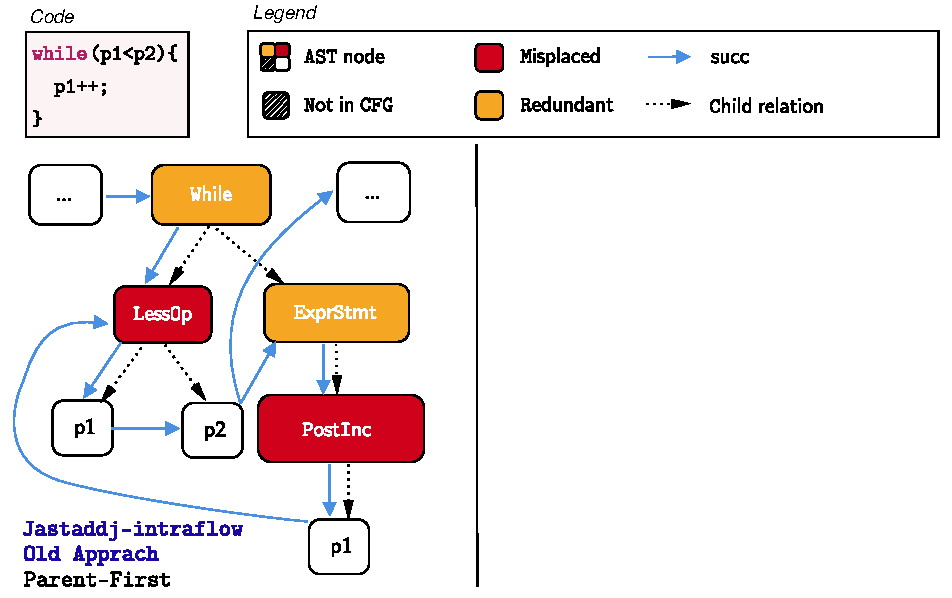
\includegraphics[scale=0.60]{img/intro2.pdf}}%
    \only<2>{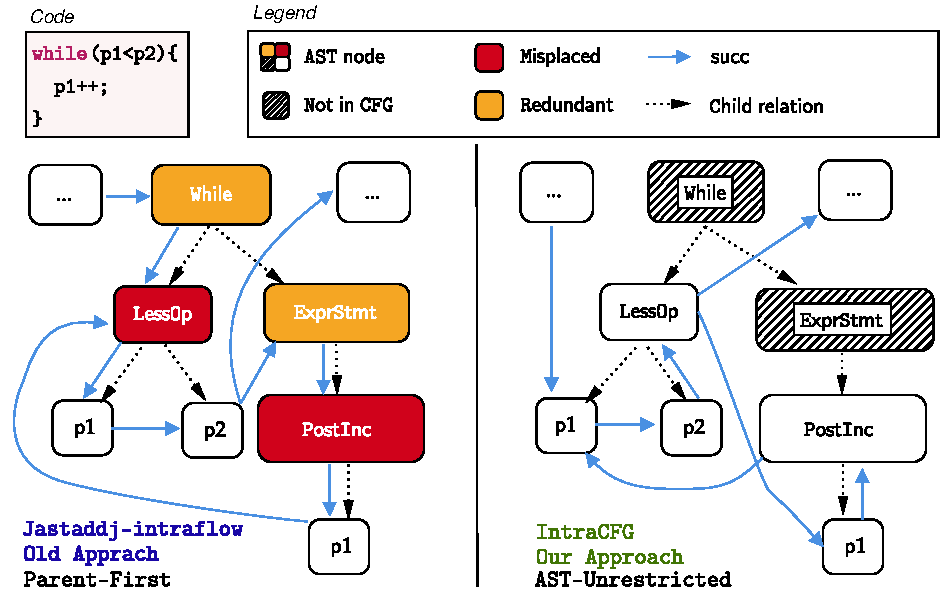
\includegraphics[scale=0.60]{img/intro1.pdf}}%
\end{center}

\end{frame}


\begin{frame}{Modular architecture}
	\hspace*{-0.9cm}
	\only<1>{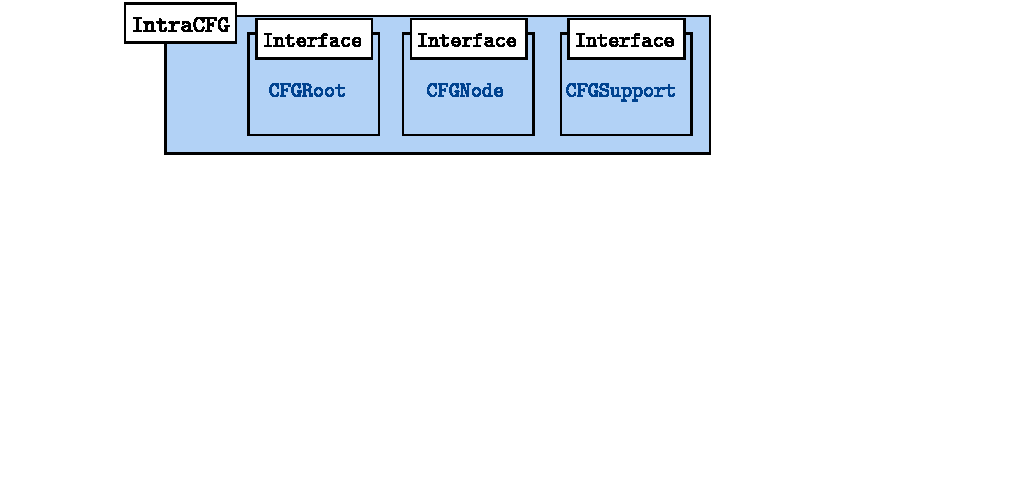
\includegraphics[scale=0.73]{img/ModularArchitecture1.pdf}}%
	\only<2>{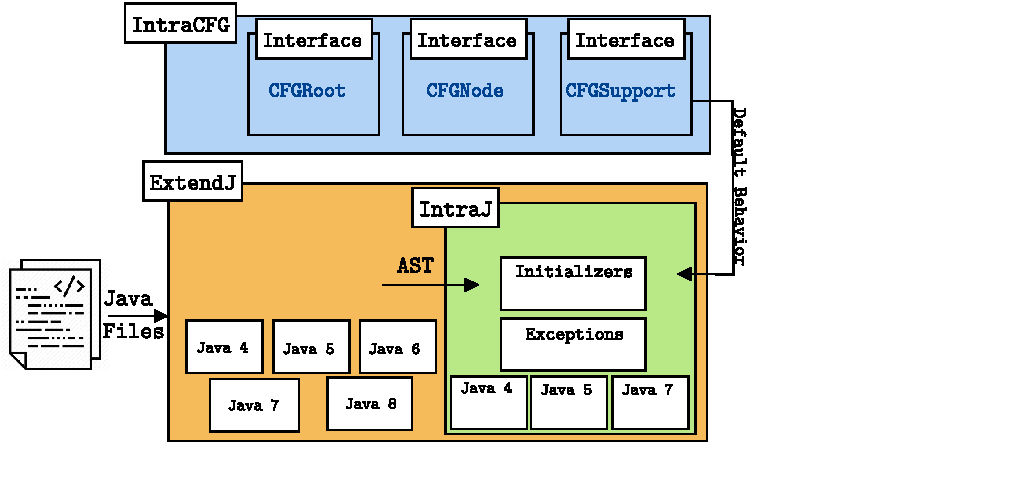
\includegraphics[scale=0.73]{img/ModularArchitecture2.pdf}}%
	\only<3>{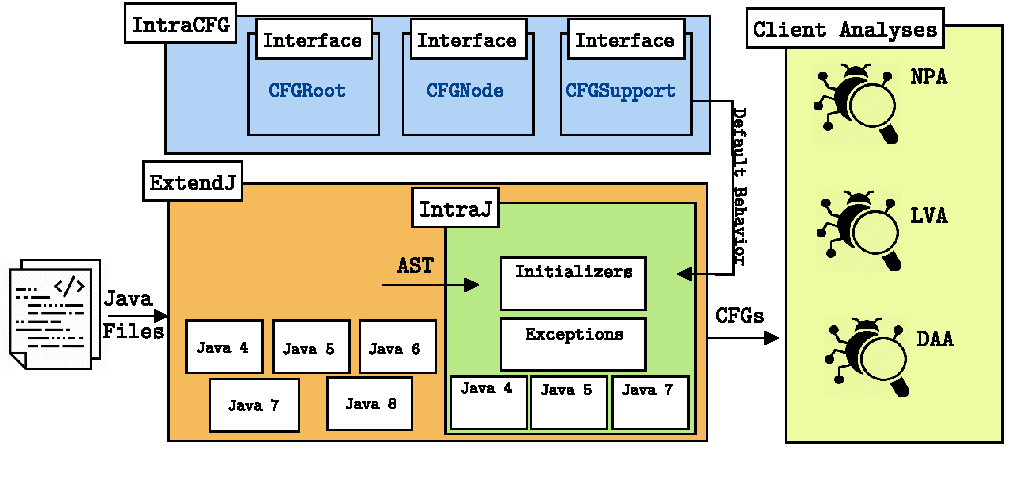
\includegraphics[scale=0.73]{img/ModularArchitecture3.pdf}}%
	\only<4>{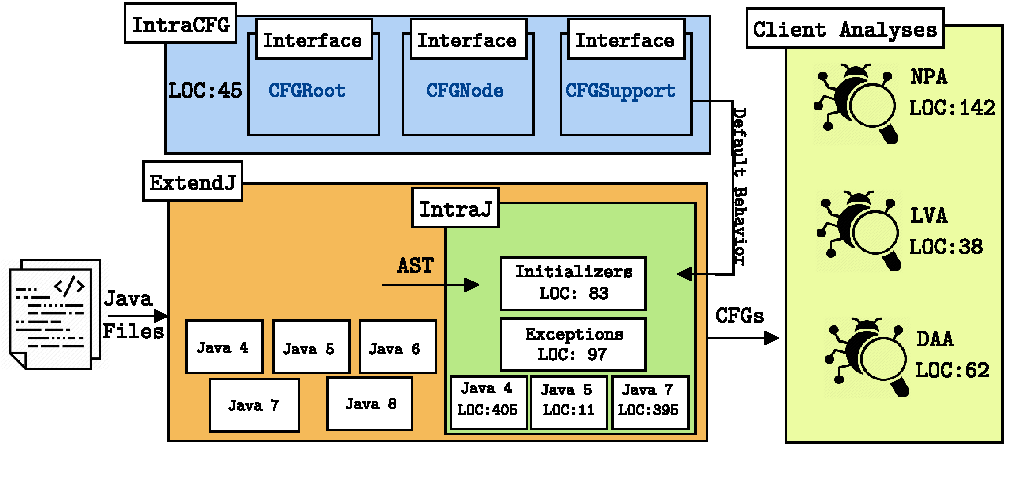
\includegraphics[scale=0.73]{img/ModularArchitecture4.pdf}}%
\end{frame}





\section{RAGs Notation}

%\begin{frame}[fragile]{Notation}
%    We defined \intracfgs\ using the RAGs formalism.
%
% \begin{onlyenv}<1>
%\phantom{test}\\
%\phantom{test}\\
%\phantom{test}\\
%\phantom{test}
% \end{onlyenv}
%
%
% \begin{onlyenv}<2>
%\begin{lstlisting}[language=JastAdd]
%syn int B.v() = 5;
%syn int C.v() = 2;
%syn int A.sum() = B.v() + C.v();
%\end{lstlisting}
%\phantom{test}
% \end{onlyenv}
%
% \begin{onlyenv}<3>
%\begin{lstlisting}[language=JastAdd]
%inh int B.v_p(); inh int C.v_p();
%eq A.getB().v_p() = A.getC().v_p();
%eq A.getC().v_p() = A.getB().v_p();
%\end{lstlisting}
%\phantom{test}
% \end{onlyenv}
%
% \begin{onlyenv}<4>
%\begin{lstlisting}[language=JastAdd]
%syn nta C.D() = new D();
%\end{lstlisting}
%\phantom{test}\\
%\phantom{test}
% \end{onlyenv}
%
% \begin{onlyenv}<5>
%\begin{lstlisting}[language=JastAdd]
%coll Set<ASTNode>  A.allChildren() [new HashSet<ASTNode>()] root A
%B contributes this to A.allChildren();
%C contributes this to A.allChildren();
%D contributes this to A.allChildren();
%\end{lstlisting}
% \end{onlyenv}
%
% \begin{onlyenv}<6>
%\begin{lstlisting}[language=JastAdd]
%syn Set<int> A.x() circular [new HashSet<>()]{
%  Set<int> res = new HashSet<int>(x);
%  if( flag ) res.add(x().size() +1);
%  return res; }
%\end{lstlisting}
% \end{onlyenv}
%
%    \begin{minipage}[h]{0.5\textwidth}
%        \only<1> {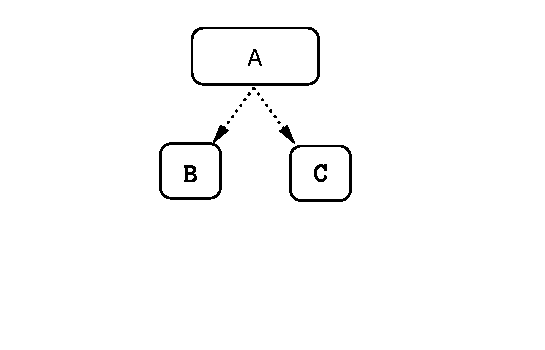
\includegraphics[scale=0.7]{img/ex1.pdf}}%
%        \only<2> {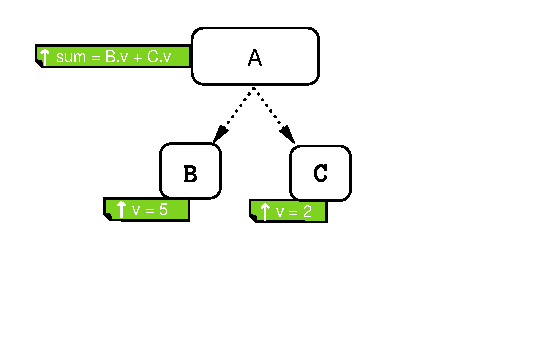
\includegraphics[scale=0.7]{img/ex2.pdf}}%
%        \only<3> {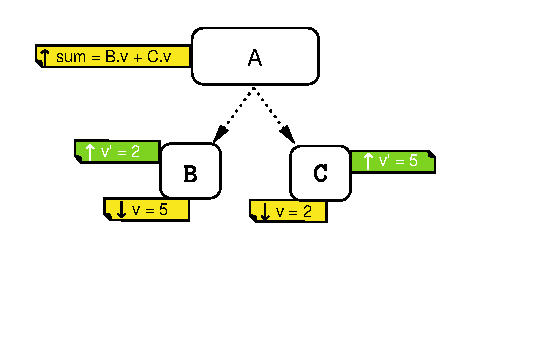
\includegraphics[scale=0.7]{img/ex3.pdf}}%
%        \only<4> {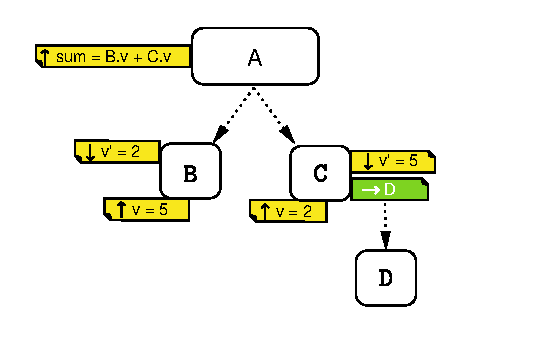
\includegraphics[scale=0.7]{img/ex4.pdf}}%
%        \only<5> {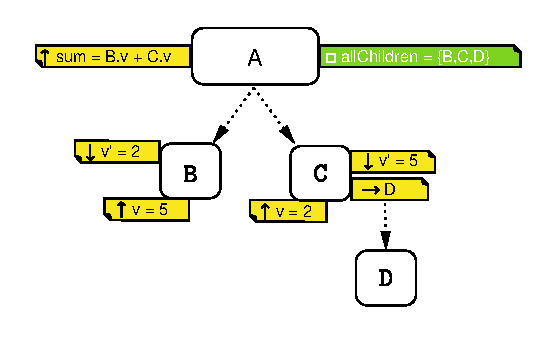
\includegraphics[scale=0.7]{img/ex5.pdf}}%
%		  \only<6-> {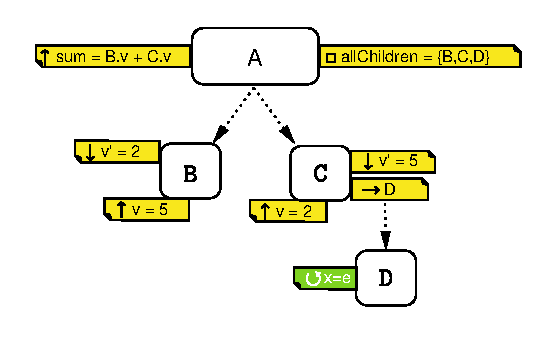
\includegraphics[scale=0.7]{img/ex6.pdf}}%
%    \end{minipage}\quad\quad\quad
%    \begin{minipage}[h]{0.3\textwidth}
%        \vspace*{-0.8cm}
%        \begin{table}[]
%            \begin{tabular}{l|l}
%            \textsc{Attribute}   & \textsc{Notation} \pause \\
%            \hline
%            \texttt{Synthesized} & \Asyn{x}=e \pause\\
%            \hline
%            \texttt{Inherited}   & \Ainh{x}=e \pause \\
%            \hline
%            \texttt{HOA}         & \Ahoa{x}=e \pause \\
%            \hline
%            \texttt{Collection}  & \Acoll{x} \pause \\
%            \hline
%            \texttt{Circular}  & \Acirc{x}=e
%            \end{tabular}
%            \end{table}
%    \end{minipage}%
%
%%\captionsetup{labelformat=empty}
%%\begin{block}{Jastadd Syntax}
%%\texttt }
%%\end{block}
%
%\end{frame}
\section{The \intracfgs\ Framework}
\begin{frame}[fragile]{Framework overview}
\vspace{0.1cm}
    \begin{minipage}[h]{0.45\textwidth}
		\only<1>{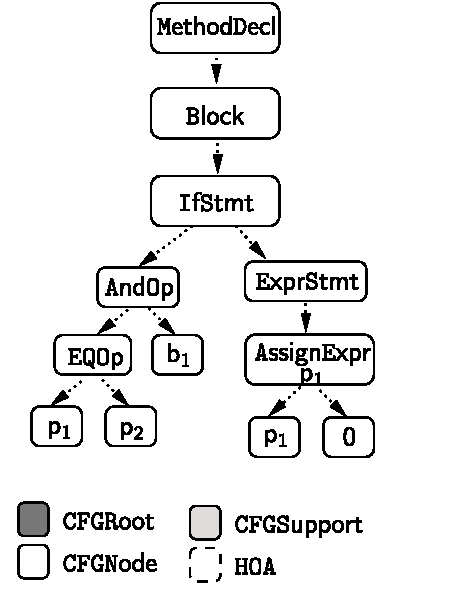
\includegraphics[scale=0.65]{img/framework1.pdf} }%
		\only<2>{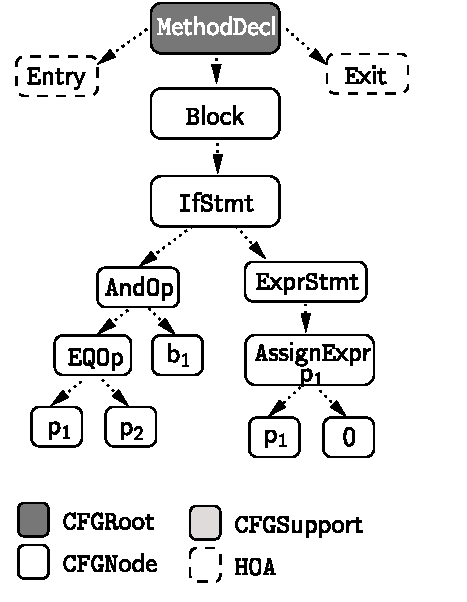
\includegraphics[scale=0.65]{img/framework2.pdf} }%
		\only<3>{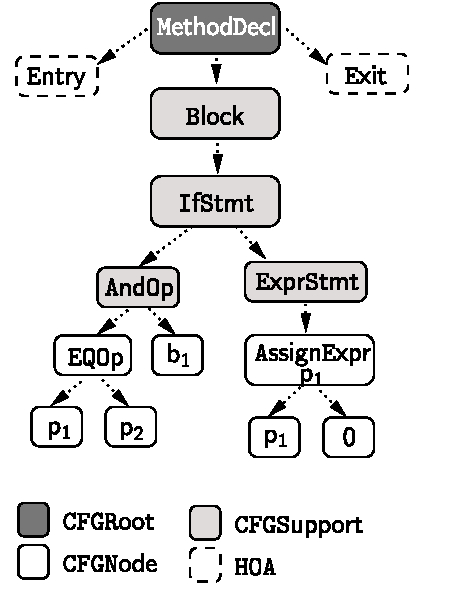
\includegraphics[scale=0.65]{img/framework3.pdf} }%
		\only<4>{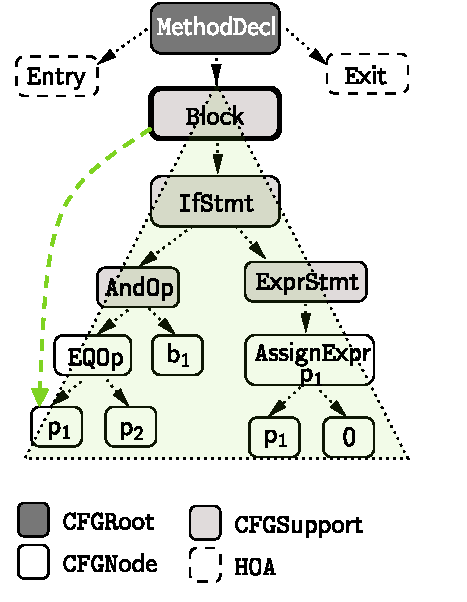
\includegraphics[scale=0.65]{img/framework3_1.pdf} }%
		\only<5>{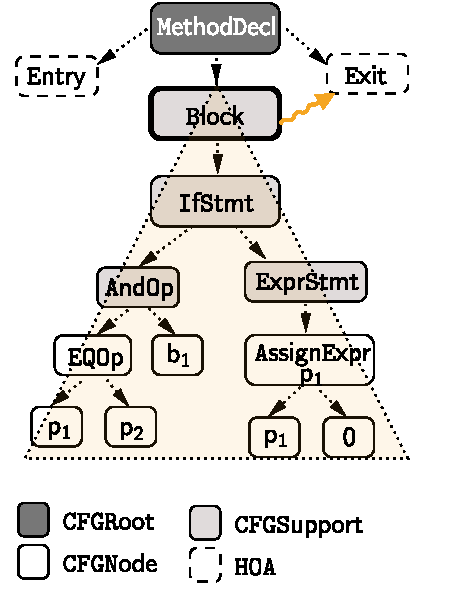
\includegraphics[scale=0.65]{img/framework3_2.pdf} }%
		\only<6>{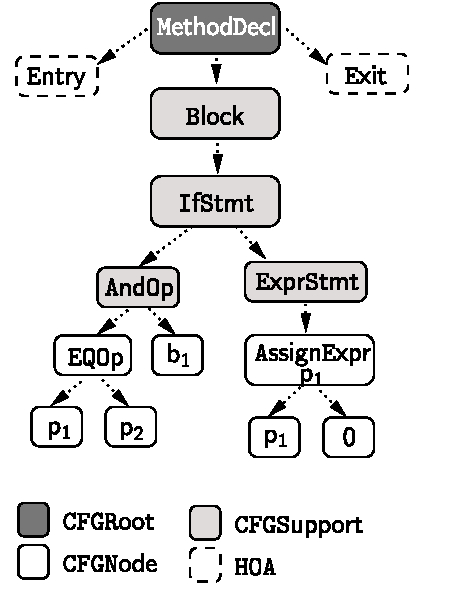
\includegraphics[scale=0.65]{img/framework3.pdf} }%
		\only<7>{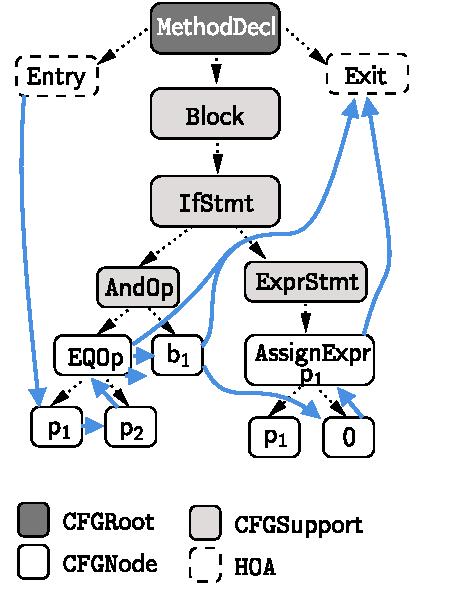
\includegraphics[scale=0.65]{img/framework4.pdf} }%
		\only<8>{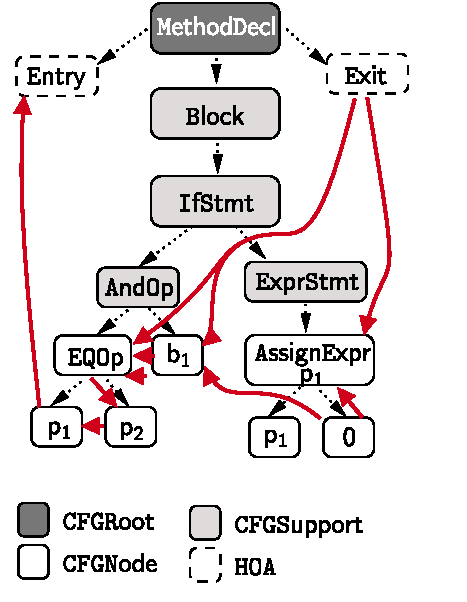
\includegraphics[scale=0.65]{img/framework5.pdf} }%
    \end{minipage}%
	\begin{minipage}[h]{0.6\textwidth}%
	\small
		  \begin{itemize}%
			\item<2-> \texttt{CFGRoot} extends the AST with two HOAs: \texttt{Entry} and \texttt{Exit}
			\item<3-> \texttt{CFGSupport} defines:
		\begin{itemize}
				\item<4-> \texttt{firstNodes}
				\item<5-> \texttt{nextNodes}
		\end{itemize}
			\item<6-> All the \texttt{CFGNode} are \texttt{CFGSupport}
%			\item \texttt{CFGNode} are the only with \texttt{succ} and \texttt{pred}
			\item<7-> Used \texttt{firstNodes} and \texttt{nextNodes} to compute the \texttt{succ} attribute
			\item<8-> The \texttt{pred} is computed as the inverse of \texttt{succ}
 		\end{itemize}%
\begin{lstlisting}[language=JastAdd]
foo(int p1, int p2, Boolean b1){
  if(p1==p2 && b1)
    p1 = 0;
}
\end{lstlisting}
    \end{minipage}%
\end{frame}



\begin{frame}{Challenges}
\begin{itemize}[<+->]
	\item We used HOAs to extend the AST with new subtrees
    \begin{minipage}[h]{0.6\textwidth}
    \begin{multicols}{2}
		\begin{itemize}
			\item Call to \texttt{close()} for resources in \textbf{Try With Resources}
			\item \textbf{Static} and \textbf{Instance}  initializers
			\item Exception-sensitivity by reifying  \textbf{Finally Blocks}.
			\item  Implicit condition in empty \textbf{For loops}
		\end{itemize}
	\end{multicols}%
\end{minipage}
	   \begin{minipage}[h]{0.3\textwidth}%
	     \onslide<5->{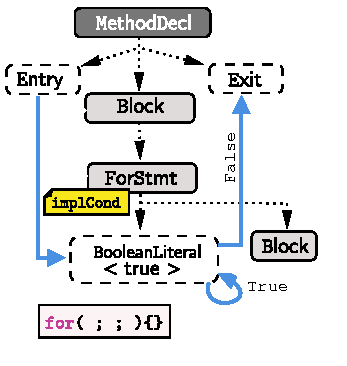
\includegraphics[scale=0.6]{img/ForExample.pdf}}%
    \end{minipage}%
	\item We used Circular attribute to compute mutually depended attributes
	\begin{itemize}
\item The attribute may depends on its own value
\item Computes a fixpoint
\end{itemize}
\end{itemize}
\end{frame}

\section{\intrajs: \intracfgs\ implementation for Java 7}
%\begin{frame}{Overview}
%    % \emphSlide{IntraJ} is an application of \emphSlide{IntraCFG}
%    \hspace*{-0.7cm}%
%    \only<1>{
\includegraphics[scale=0.5]{img/intraj1.pdf}}%
%    \only<2>{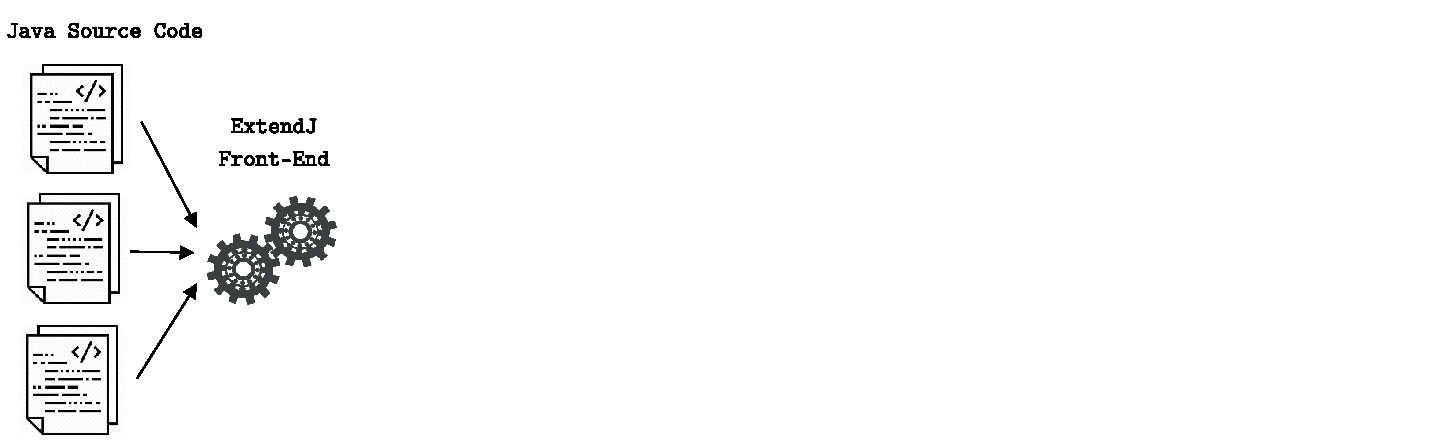
\includegraphics[scale=0.5]{img/intraj2.pdf}}%
%    \only<3>{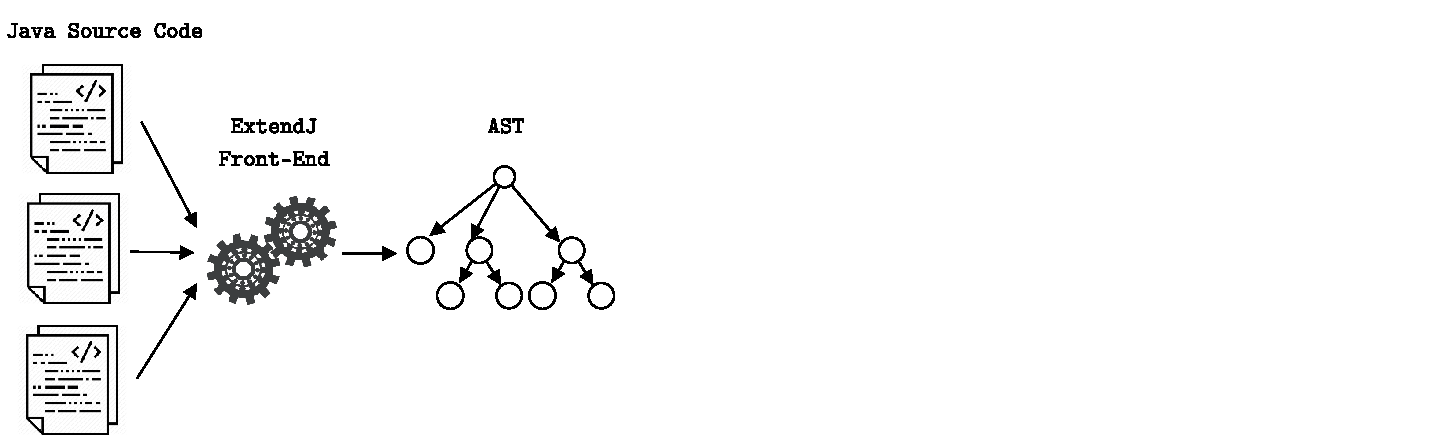
\includegraphics[scale=0.5]{img/intraj3.pdf}}%
%    \only<4>{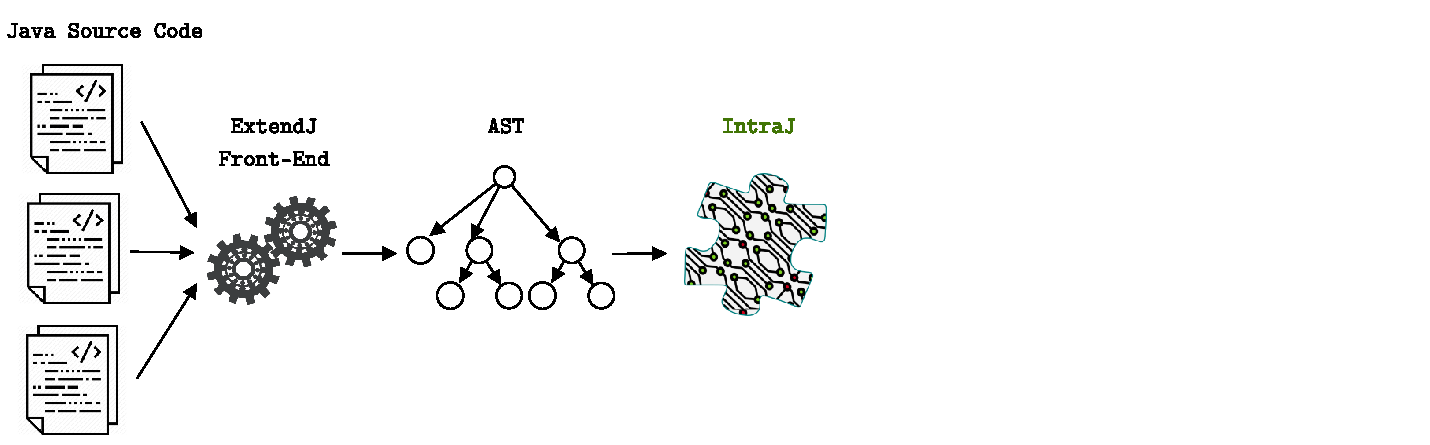
\includegraphics[scale=0.5]{img/intraj4.pdf}}%
%    \only<5>{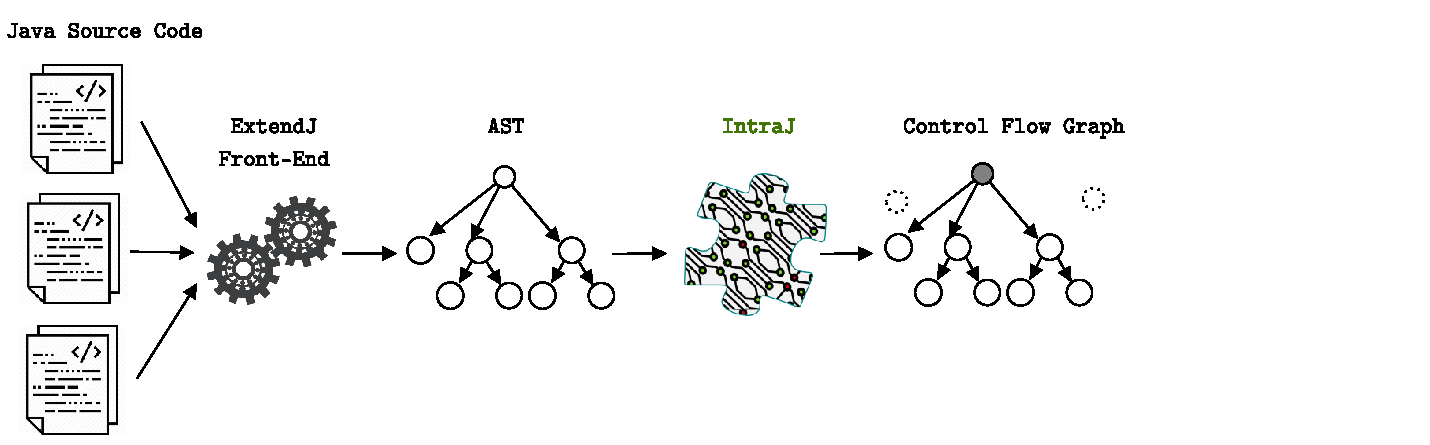
\includegraphics[scale=0.5]{img/intraj51.pdf}}%
%    \only<6>{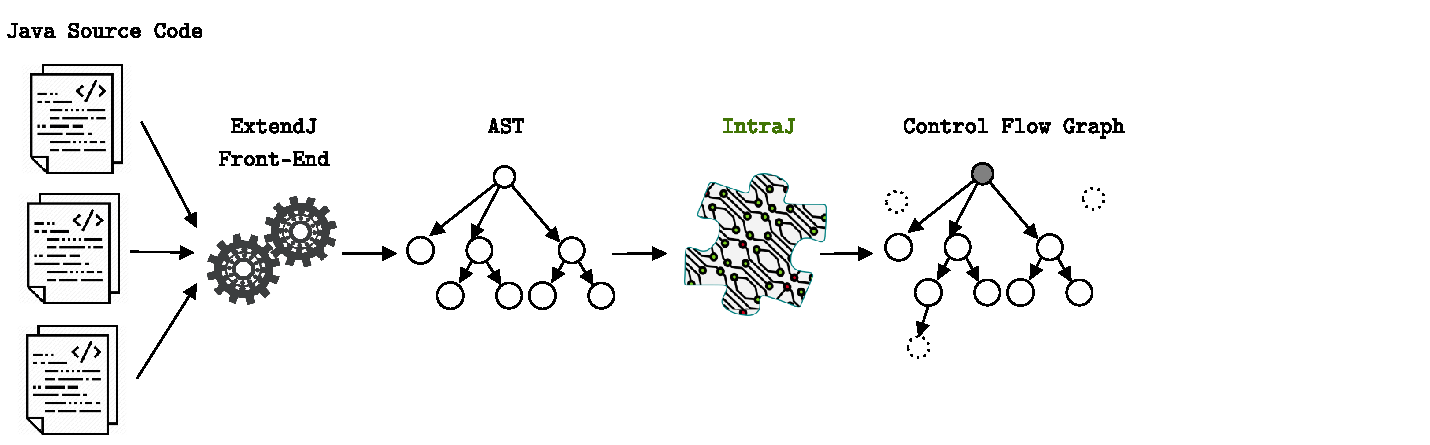
\includegraphics[scale=0.5]{img/intraj52.pdf}}%NTA
%    \only<7>{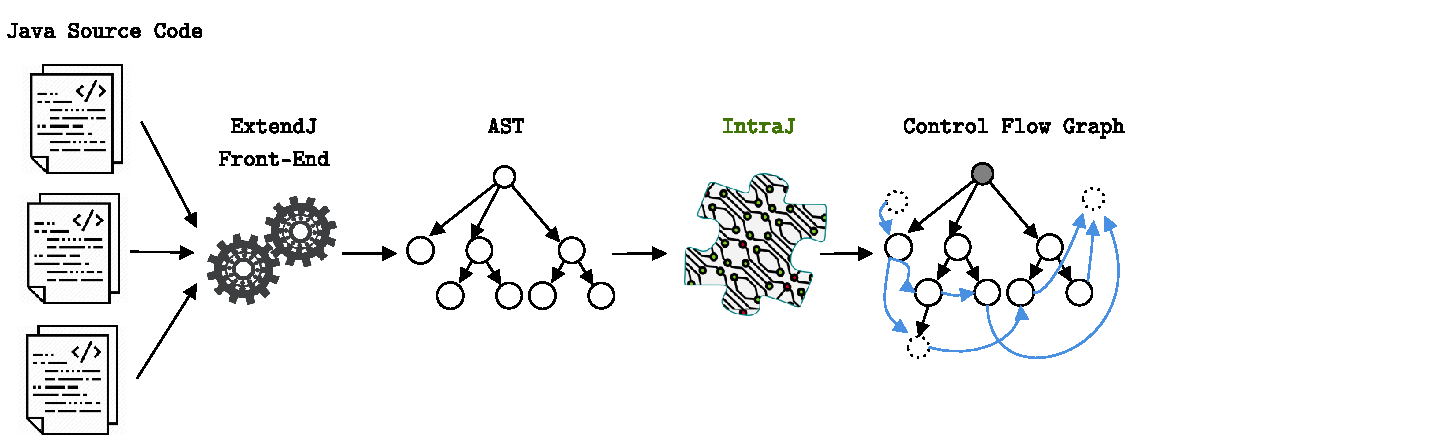
\includegraphics[scale=0.5]{img/intraj53.pdf}}%succ
%    \only<8>{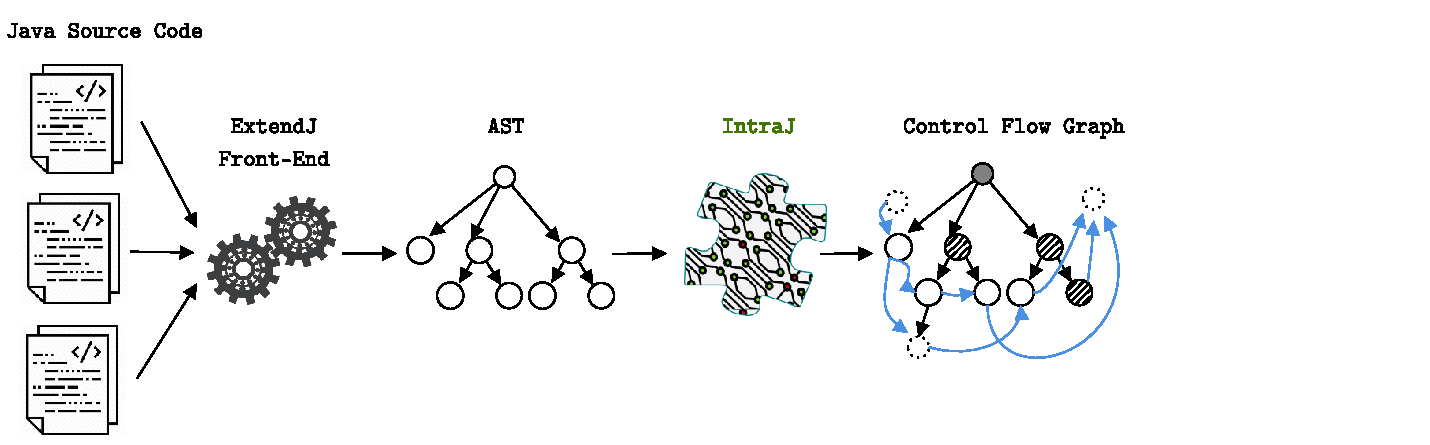
\includegraphics[scale=0.5]{img/intraj54.pdf}}%CFGSupport
%    \only<9>{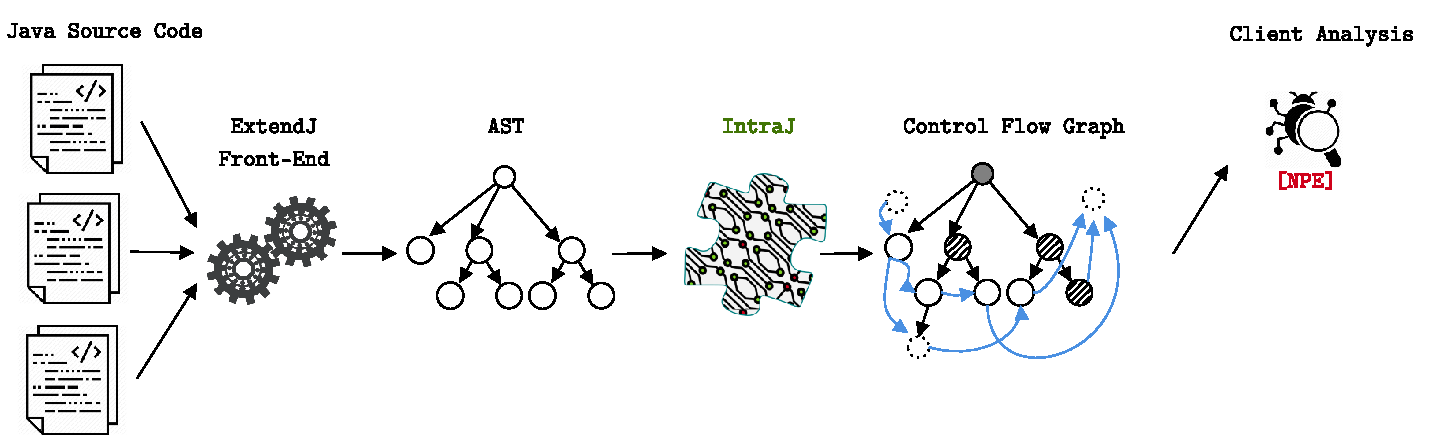
\includegraphics[scale=0.5]{img/intraj6.pdf}}%
%    \only<10>{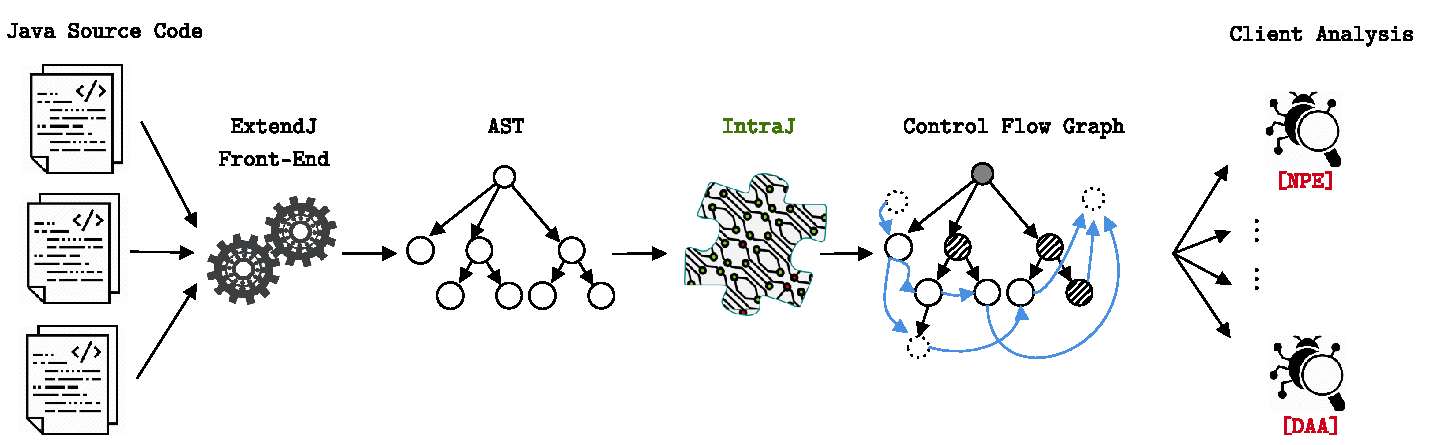
\includegraphics[scale=0.5]{img/intraj7.pdf}}%
%    \begin{multicols}{2}
%        \begin{itemize}
%            \item<2-> \emphSlide{IntraJ} is an extension of \lowEmph{ExtendJ} Java Compiler
%            \item<4-> \emphSlide{IntraJ} superimpose the CFGs on the attributed AST generated by ExtendJ
%            \item<6-> \emphSlide{Precision}: HOAs to reify implicit facts
%            \item<8-> \emphSlide{Minimality}: redundant nodes are excluded
%        \end{itemize}
%    \end{multicols}
%\end{frame}
%
%\begin{frame}{Overview}
%\emphSlide{IntraJ} is an application of the \emphSlide{IntraCFG} framework. We implemented IntraJ as an extension of the \lowEmph{ExtendJ} Java compiler.
%
%Our two main goals were:
%	\begin{itemize}
%		\item Minimality: build concise CFG by excluding AST nodes that do not correspond to any \textit{runtime action}.
%		\item High Precision: the constructed CFGs should capture most program \textit{details}.
%	\end{itemize}
%\end{frame}
%
%


\section{Evaluation}
\begin{frame}[fragile]{Client analyses}
    We validate \intrajs\ by implementing three different dataflow analyses:
    \begin{itemize}\small
        \item {\color<2->{ForestGreen}{\texttt{NullPointerAnalysis}}} - \emphSlide{NPA} \hfill \textbf{MAY - FORWARD }
        \item \texttt{LiveVariableAnalysis} - \emphSlide{LVA} \hfill \textbf{MAY - BACKWARD}
        \item \texttt{DeadAssignmentAnalysis} - \emphSlide{DAA} \hfill uses \emphSlide{LVA}
    \end{itemize}
\vspace{0.5cm}
\hspace{-0.8cm}
	    \begin{minipage}[h]{0.4\textwidth}
\onslide<2->{
	     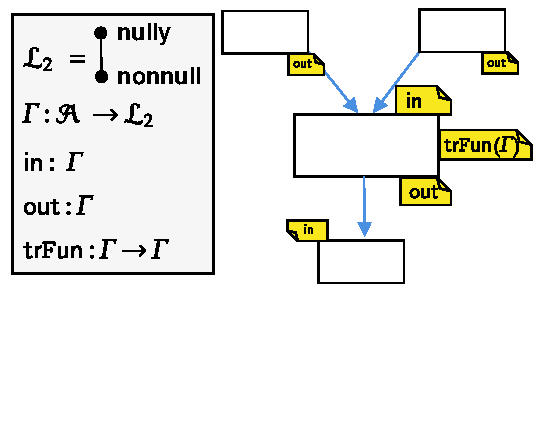
\includegraphics[scale=0.65]{img/npa.pdf}%
}
    \end{minipage}\hfill%
	    \begin{minipage}[h]{0.5\textwidth}
\begin{onlyenv}<3->


\footnotesize
$\bullet$\ Default behaviour for \texttt{CFGNodes}
\begin{lstlisting}[frame=none,language=JastAdd]
trFun(@$\Gamma$@){
  return @$\Gamma$@;
}
\end{lstlisting}
 $\bullet$\ Specialised behaviour for \texttt{AssignExpr}
\begin{lstlisting}[frame=none, language=JastAdd]
trFun(@$\Gamma$@){
  if(rhs.mayBeNull())
    @$\Gamma$@.put(lhs.decl(),nully);
  else
    @$\Gamma$@.put(lhs.decl(),nonnull);
  return @$\Gamma$@;
}
\end{lstlisting}

\end{onlyenv}
    \end{minipage}%

\end{frame}
%\begin{frame}{Overview}
%We conducted two different studies:\vspace{0.2cm}
%	\begin{itemize}
%		\item We compared the size of the CFGs constructed by \intrajs\ against the ones constructed by the earlier  RAG-based framework \lowEmph{Jastaddj-intraflow} (JJI)\vspace{0.1cm}
%
%		\item We compared the precision and performance of \intrajs\  against the highly-tuned  industrial static checker \lowEmph{SonarQube} (SQ)
%
%	\end{itemize}
%
%\onslide<2->{
%\begin{table}
%\centering
%\begin{tabular}{l|l|l|l|l}
%     & \textsc{Antlr}                    & \textsc{Pmd}                      & \textsc{Jfc}                      & \textsc{Fop}                      \\
%\hline
%\textsc{LOC}  & \multicolumn{1}{c|}{33K} & \multicolumn{1}{c|}{49K} & \multicolumn{1}{c|}{95K} & \multicolumn{1}{c}{97K}
%\end{tabular}
%\end{table}
%}
%\end{frame}

\begin{frame}{Overview}
\begin{center}
\only<1>{%

\includegraphics[scale=0.7]{img/eval1.pdf}%
}%
\only<2>{%

\includegraphics[scale=0.7]{img/eval15.pdf}%
}%
\only<3>{%
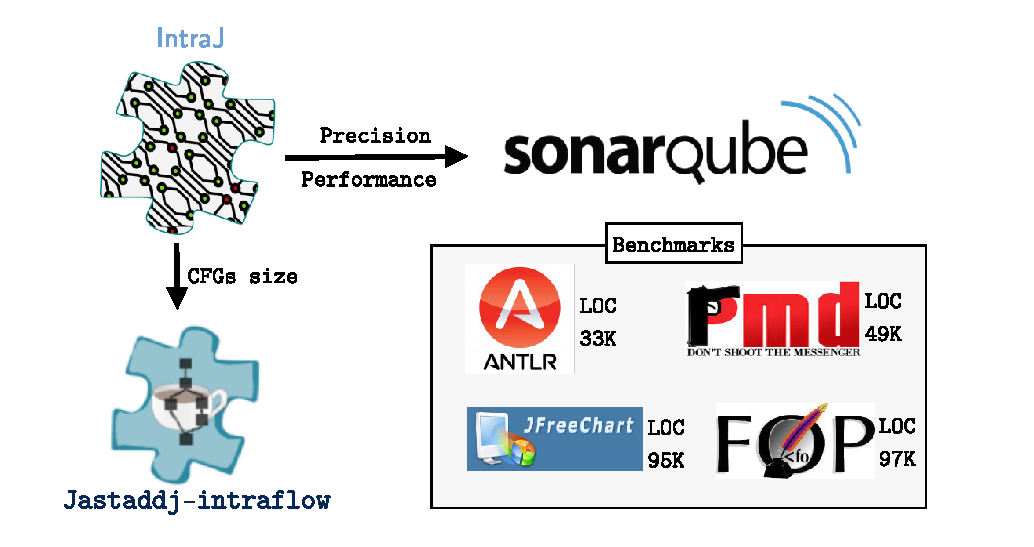
\includegraphics[scale=0.7]{img/eval2.pdf}%
}%
\end{center}
\end{frame}


\begin{frame}[fragile]{Benchmark Projects}
\begin{center}
  \intrajs\ reduces the CFGs  size by 30\% - 40\%
  \begin{table}
\centering
\begin{tabular}{ccccc}
Benchmark & Qty & \intraj& JJI & \% \\
\hline
\multirow{2}{*}{\textsc{Antlr}} & \textsc{Nodes} & 76$^\cdot$925 & 116$^\cdot$523 & \emphSlide{-39.9} \\
\cline{2-5}
 & \textsc{Edges} & 85$^\cdot$028 & 136$^\cdot$528 & \emphSlide{-37.7} \\
\hline
\multirow{2}{*}{\textsc{Pmd}} & \textsc{Nodes} & 103$^\cdot$739 & 182$^\cdot$864 & \emphSlide{-43.2} \\
\cline{2-5}
 & \textsc{Edges} & 108$^\cdot$639 & 202$^\cdot$842 & \emphSlide{-46.4} \\
\hline
\multirow{2}{*}{\textsc{Jfc}} & \textsc{Nodes} & 219$^\cdot$419 & 331$^\cdot$368 & \emphSlide{-33.7} \\
\cline{2-5}
 & \textsc{Edges} & 220$^\cdot$256 & 363$^\cdot$642 & \emphSlide{-39.4} \\
\hline
\multirow{2}{*}{\textsc{Fop}} & \textsc{Nodes} & 239$^\cdot$096 & 347$^\cdot$125 & \emphSlide{-31.1} \\
\cline{2-5}
 & \textsc{Edges} & 240$^\cdot$068 & 379$^\cdot$269 & \emphSlide{-36.6} \\
\hline
\end{tabular}
\end{table}
By removing all the {\color{orange}redundant} nodes
\end{center}
\end{frame}



\begin{frame}[fragile]{\intrajs\  vs \lowEmph{SonarQube}}
	We evaluated \emphSlide{IntraJ} against \lowEmph{SonarQube}
		\only<1>{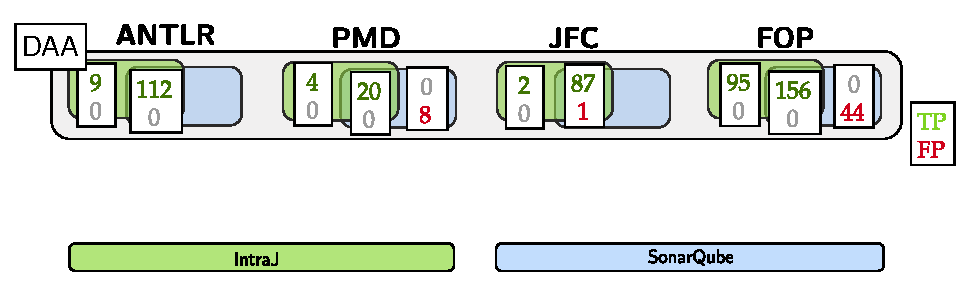
\includegraphics[scale=0.7]{img/precision1.pdf}}
		\only<2>{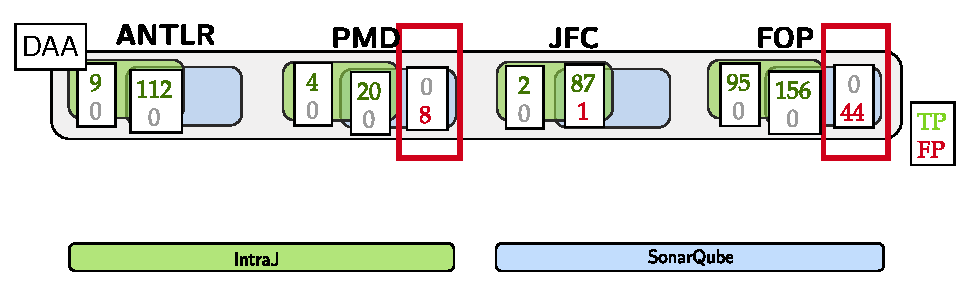
\includegraphics[scale=0.7]{img/precision2.pdf}}
		\only<3>{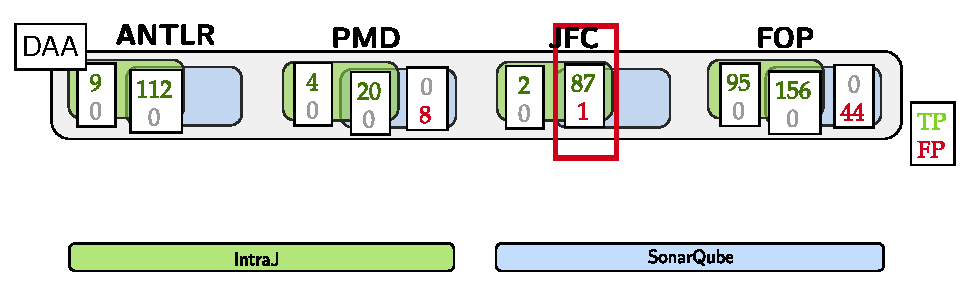
\includegraphics[scale=0.7]{img/precision3.pdf}}
		\only<4>{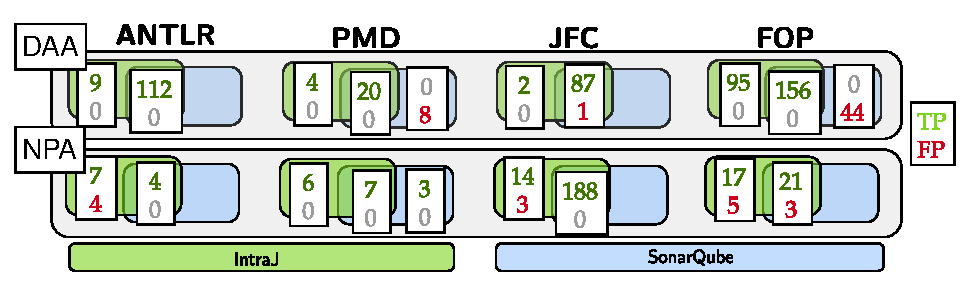
\includegraphics[scale=0.7]{img/precision4.pdf}}
		\only<5->{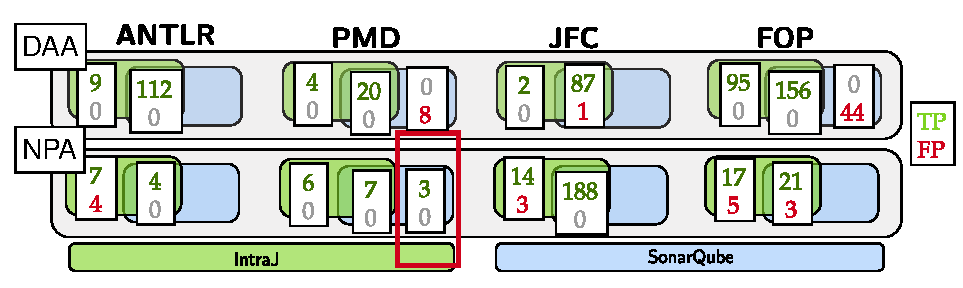
\includegraphics[scale=0.7]{img/precision5.pdf}}


\onslide<6->{
\begin{table}
\centering
\begin{tabular}{|c|r|r|r|r|r|r|}
\hline
\multirow{2}{*}{Benchmark } & \multicolumn{2}{c|}{\textbf{\color<7>{ForestGreen}{Baseline}} (s)}               & \multicolumn{2}{c|}{ \color<8>{ForestGreen}{\textbf{DAA}} (s)}                     & \multicolumn{2}{c|}{\textbf{ \color<9>{ForestGreen}{NPA}} (s)}                     \\
\cline{2-7}
                            & \multicolumn{1}{c|}{IntraJ} & \multicolumn{1}{c|}{SQ} & \multicolumn{1}{c|}{IntraJ} & \multicolumn{1}{c|}{SQ} & \multicolumn{1}{c|}{IntraJ} & \multicolumn{1}{c|}{SQ}  \\
\hline
\textbf{ANTLR}              & \color<7>{ForestGreen}{2.14}                        &  \color<7>{red}{4.91}                    &  \color<8>{red}{0.53}                        & \color<8>{ForestGreen}{0.24}                   &  \color<9>{ForestGreen}{0.90}                             &  \color<9>{red}{12.35}                    \\
\hline
\textbf{PMD}                &  \color<7>{ForestGreen}{3.56}                     & \color<7>{red}{10.76}                  &  \color<8>{red}{0.47}                        &  \color<8>{ForestGreen}{0.18}                   &  \color<9>{ForestGreen}{0.80}                        &   \color<9>{red}{12.40}                    \\
\hline
\textbf{JFC}                &  \color<7>{ForestGreen}{4.29}                       &\color<7>{red}{10.81}                &  \color<8>{red}{0.75}                        &  \color<8>{ForestGreen}{0.24}                    &  \color<9>{ForestGreen}{1.62}                        &   \color<9>{red}{10.71}                    \\
\hline
\textbf{FOP}                &  \color<7>{ForestGreen}{ 4.42}                     & \color<7>{red}{17.20}                  &  \color<8>{red}{0.67}                       &  \color<8>{ForestGreen}{0.34}                    &  \color<9>{ForestGreen}{1.42}                        &   \color<9>{red}{19.25}                    \\
\hline
\end{tabular}
\end{table}
}
\end{frame}




%    \begin{minipage}{0.4\textwidth}
%    \begin{lstlisting}[ language=Java, label=listing:npaTruePositiveIntraJ, basicstyle=\tiny]
%void bar(boolean flag){
%  Object o = null;
%  if (flag)
%    o = new Object();
%  if (flag)
%    println(o.toString());
%}
%    \end{lstlisting}
%    \end{minipage}%
%	\hfill
%    \begin{minipage}{0.4\textwidth}
%    \begin{lstlisting}[ language=Java, label=listing:npaTruePositiveSQ, basicstyle=\tiny]
%void foo(){
%  Object rs = getRS();
%  if(rs==null)
%      // rs can be null
%      panic(); //exit(1)
%  println(rs.toString());
%}
%    \end{lstlisting}
%    \end{minipage}%\
\section{Conclusions}
\begin{frame}{\intracfgs\ \& \intrajs}
   We presented \intracfgs, a language independent RAGs framework that overcomes the limitations of earlier approaches:
	\begin{itemize}
	\item \textbf{High precision}
	\item \textbf{$\ge$30\% fewer nodes}
	\item\textbf{Better performance} for large code bases
\end{itemize}
\onslide<2->{
Moreover, we presented:}
    \begin{itemize}
        \item<2-> \intrajs,an instance of \intracfgs\ for Java 4-7 \\ \vspace{0.1cm}
        \item<3-> Concise code for CFG and client analyses \\ \vspace{0.1cm}
        \item<4-> Competitive to  \lowEmph{SonarQube} \\ \vspace{0.1cm}
    \end{itemize}

\begin{center}
\onslide<5->{\textsc{\emphColorSlide{Thank you for your attention!}}}
\end{center}
\end{frame}

%No page Numbering
\setbeamercolor{headline}{fg=white,bg=black}
\setbeamertemplate{headline}{
	\begin{beamercolorbox}[wd=1.0\paperwidth,left,ht=38pt,dp=1ex]{headline}
	\end{beamercolorbox}
	\vspace*{2.3pt}
	\color{black!30!white}\rule{\paperwidth}{2pt}
}


\end{document}